\documentclass{subfiles}

\begin{document}

  \chapter{Sistema básico}
  \label{chap:2}

        \section{Estructura}
        \label{sec:2.1}
        Debido a la clara repartición de tareas en cada sección del código, se ha pretendido aplicar una separación tipo Modelo-Vista-Controlador en la aplicación, de manera que todo esté visiblemente separado y se pueda utilizar un sistema de orientación a objetos en toda la parte escrita en \js.

        \paragraph{}
        La primera sección a comentar sería el Modelo. En esta aplicación, tal y como se ha planteado el desarrollo y teniendo en cuenta qué librerías externas se han incorporado y cómo se han utilizado, se ha tratado a estas como si fueran el propio Modelo. Así, nuestra información es en sí las librerías externas añadidas, que serán además las que se encarguen de cargar los datos estáticos de servidor: los modelos en 3D y las grabaciones de las voces de estos.

        \paragraph{}
        La segunda sección sería la Vista. En este caso, la Vista de esta aplicación constaría únicamente de un HTML llamado \textit{index}, que sería además la \textit{landing page} de la aplicación. Sobre esta misma página será sobre la que se colocará más tarde un \textit{<<canvas>>}, que es el elemento HTML que permite mostrar elementos gráficos de manera dinámica a través de \js. Utilizando este último podremos mostrar las imágenes captadas a través de la cámara del dispositivo móvil y mezclarlas con los modelos en 3D para generar nuestra \ra.

        \paragraph{}
        Por último, la sección restante sería el Controlador. En este, se procesan todos los eventos generados por el usuario, además de tratar toda la información que se recibirá de los sensores del dispositivo para poder generar las imágenes de manera verosímil. En este se ubicará un bucle que se ocupará de obtener la imagen a mostrar, mezclarla con el modelo en 3D, renderizar la imagen y situarla en la vista, todo esto de la manera más fluida posible para que el espectador no tenga impresiones que entorpezcan la experiencia de usuario.

        \paragraph{}
        Además, esta almacenará también información de la sesión necesaria para el correcto procesamiento del sistema, tales como los modelos en 3D cargados, la referencia al objeto de \js con el \textit{<<canvas>>} antes mencionado, la posición del usuario y otros datos necesarios para el funcionamiento del sistema que serán mencionados a lo largo de esta memoria.

        \paragraph{}
        Es importante mencionar que, a pesar de que se ha tratado a este sistema como un Modelo-Vista-Controlador y se le ha presentado como tal, sería más justo tratar a la aplicación como si utilizara el patrón Modelo-Vista-Presentador \cite{web:mvp} por varias razones.

        \paragraph{}
        La primera es que no tenemos constancia de cómo almacenan estas librerías las pocas referencias que se le entregan a la Vista y, aún manteniendo esta referencia como si lo tratara como la Vista en este tipo de patrones, no parece realizar cambios sobre esta de manera directa.

        \paragraph{}
        La segunda es que las actualizaciones se realizan directamente desde el Controlador, siendo necesario realizar desde este último acciones explícitas para actualizar la apariencia de la vista, como por ejemplo el renderizado de la imagen a mostrar en pantalla.

        \paragraph{}
        Por último y más importante, es necesario que todos los cambios estén revisados en el bucle que se genera en el Controlador, el cual se tratará más adelante. Esto obliga a este último a solicitar información continuamente a las librerías, hacer cálculos y mostrarlos en pantalla, mientras está atento a los eventos de los usuarios.

        \begin{figure}
        \centering
        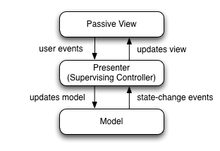
\includegraphics[width=0.5\textwidth]{img/mvp.png}
        \caption{Representación gráfica del patrón Modelo-Vista-Presentador. Imagen obtenida de Wikipedia.}
        \label{fig:mvp}
        \end{figure}

        \paragraph{}
        Por todo esto, y dado que la lógica de negocio está separada de la interfaz de usuario, la estructura se corresponde con el patrón Modelo-Vista-Presentador. Sin embargo, dado que desde el inicio del proyecto se trató cada parte como el clásico Modelo-Vista-Controlador, y dado que el Modelo-Vista-Presentador proviene de este último, cada parte será nombrada como si lo fuera, aún siendo conscientes de las diferencias.

        \section{Sesión WebXR}
        \label{sec:2.2}

        La primera herramienta que será necesario inicializar es una instancia de Sesión de \webxr. La Sesión de \webxr, llamada \textit{XRSession} \cite{web:xrsession}, es el objeto de la librería \webxr que provee de las funcionalidades más básicas, así como de utilidades extra que serán implementadas a lo largo del desarrollo de la aplicación. Esta interfaz pretende representar la propia actividad que llevará a cabo el usuario mientras observa la \ra, por lo que tendrá funciones orientadas a iniciar, mantener y terminar esta actividad.

        \paragraph{}
        Para ser inicializado, el objeto Sesión tiene varios requisitos que se deben cumplir \cite{web:webxrrequirements} para evitar problemas de seguridad. Los dos requisitos mencionados por la documentación de \arcore son:

        \begin{itemize}
            \item {El servidor que ofrezca el servicio debe tener una conexión a través de un entorno seguro. \webxr considerará segura una comunicación que se transmita a través del protocolo \textit{HTTPS} y/o que se ubique en \textit{localhost}}.
            \item {El cliente debe utilizar un navegador compatible con WebXR. A fecha de este documento, solo existen tres navegadores para dispositivos móviles que cumplan este requisito \cite{web:webxrcompatibility}: \googlechrome para \android a partir de la versión 79, \textit{Opera} para \android a partir de la versión 57 y \textit{Samsung Internet} a partir de la versión 11.2. Además, el dispositivo que lo lance debe soportar la aplicación \arcore.}
        \end{itemize}

        Además de esto, la sesión se debe iniciar a través de lo que el sistema debe interpretar que es un evento de usuario. Esto quiere decir que la sesión no se puede generar automáticamente o nada más cargarse la página, sino que debe ser el usuario pulsando un botón o realizando una acción consciente el que lance la solicitud de inicio de sesión de \ra.

        \paragraph{}
        Teniendo en mente estas condiciones, se planteó que la Vista debía ser una interfaz sencilla que contuviese un botón que debiera accionar el usuario para iniciar la sesión, siendo en las versiones más prematuras un botón simple sin ningún tipo de customización. En las versiones más avanzadas, se generó un fichero \textit{CSS} que personalizara la \textit{landing page} de manera que, además de tener los colores de la empresa, tuviese un aspecto más amigable para el usuario.

        \begin{figure}
        \centering
        
\includegraphics[width=0.25\textwidth]{img/landing_page.jpg}
        \caption{Imagen de la \textit{landing page} definitiva de la aplicación web.}
        \label{fig:landing_page}
        \end{figure}

        %% comentar llamada del botón, lanzamiento de la aplicacion para cumplir condiciones, server https,
        
        \section{Procesado iterativo}
        \label{sec:2.x}

        Para poder asignar a cada fotograma, así como hacer los propios cálculos en cada momento de la ubicación y movimientos de las figuras que vamos a insertar llegado el momento, es necesario crear un bucle que dure tanto tiempo como el usuario vaya a permanecer en la aplicación. En cada una de las iteraciones, la aplicación solicitará al hardware del dispositivo móvil la imagen captada a través de su cámara, de disponer de una.

        \paragraph{}
        Para evitar que el sistema se ralentice, las solicitudes de fotogramas se realizan de una forma un tanto particular. En lugar de utilizar un bucle estándar como pueda ser uno tipo <<for>> o <<while>>

\end{document}
